\documentclass[a4paper,8pt]{extarticle} % 使用更小的字号
\usepackage[top=0.4cm,bottom=0.4cm,left=0.4cm,right=0.4cm]{geometry} % 设置页边距
\usepackage{multicol} % 多栏排版
\usepackage{amsmath}
\usepackage{amssymb}
\usepackage{physics}
\usepackage{xcolor}
\usepackage[UTF8]{ctex} % Required for inserting images
\usepackage{longtable}
\usepackage{array}
\usepackage{tabularx}
\usepackage{graphicx}
\usepackage{float}
\usepackage{listings}
\usepackage[hidelinks]{hyperref}
\usepackage{titlesec}
\usepackage{tocloft}
\usepackage{parskip} % 用于段落格式控制

% 取消首行缩进
\setlength{\parindent}{0pt}
% 设置行距
\linespread{0.9}
% 设置公式间距
\setlength{\abovedisplayskip}{2pt}
\setlength{\belowdisplayskip}{2pt}
\setlength{\abovedisplayshortskip}{2pt}
\setlength{\belowdisplayshortskip}{2pt}

% 设置段落间距
\setlength{\parskip}{0.4ex}

% 定义蓝色、红色文本、背景色
\newcommand{\bluetext}[1]{\textcolor{blue}{#1}}
\newcommand{\redtext}[1]{\textcolor{red}{#1}}
\newcommand{\greentext}[1]{\textcolor{green}{#1}}
\newcommand{\yellowback}[1]{\colorbox{yellow}{#1}}

% 定义粗体
\newcommand{\black}[1]{\textbf{#1}}

% 优化多栏环境的分页设置
\raggedcolumns
\begin{document}
\begin{multicols}{3}
\setlength{\columnsep}{0.1cm} 

\redtext{定态微扰论}

\bluetext{微扰方程}:原方程:$(\hat{H}^{(0)} + \hat{H}')\psi_n = E_n\psi_n$;\\
零级方程:$\hat{H}^{(0)}\psi_n^{(0)} = E_n\psi_n^{(0)}$;\\
一级方程:$(\hat{H}^{(0)} - E_n^{(0)})\psi_n^{(1)} = -(\hat{H}' - E_n^{(1)})\psi_n^{(0)}$;\\
二级方程:$(\hat{H}^{(0)} - E_n^{(0)})\psi_n^{(2)} = -(\hat{H}' - E_n^{(1)})\psi_n^{(1)} + E_n^{(2)}\psi_n^{(0)}$。

\bluetext{无简并的微扰论}:能级一级修正:$E_n^{(1)} = H_{nn}' = \int \psi_n^{(0)*} \hat{H}'\psi_n^{(0)} \mathrm{d}\tau$;能级二级修正:$E_n^{(2)} = \sum_k \frac{|H_{kn}'|^2}{E_n^{(0)}-E_k^{(0)}}$;波函数一级修正:$\psi_n^{(1)}(x) = \sum_{k\neq n} \frac{H_{kn}'}{E_n^{(0)}-E_k^{(0)}} \psi_k^{(0)}(x)$。

\greentext{推导过程}

\bluetext{带有简并的微扰论}:

一级方程:$(\hat{H}^{(0)} - E_n^{(0)})\psi_{nl}^{(1)} = -(\hat{H}' - E_{nl}^{(1)})\psi_{nl}^{(0)}$;零级波函数:$\psi_{nl}^{(0)} = \sum_{j=1}^k c_{jl}^{(0)} \phi_{nj}^{(0)}$;一级波函数:$\psi_{nl}^{(1)} = \sum_m c_{ml}^{(1)}\phi_m^{(0)}$,其中 $c_{ml}^{(1)} = \frac{\int \phi_m^{(0)*} \hat{H}' \psi_{nl}^{(0)} \mathrm{d}\tau}{E_n^{(0)}-E_m^{(0)}}$;一级能级修正:$E_{nl}^{(1)}$ 为 $H'$ 对应子阵的本征值;二级能级修正:$E_{nl}^{(2)} = \sum_m \frac{|\int \phi_m^{(0)*} \hat{H}' \psi_{nl}^{(0)} \mathrm{d}\tau|^2}{E_n^{(0)}-E_m^{(0)}}$。

\bluetext{zeeman效应}:

实验证明,在外磁场中原子的能级会发生分裂。理论解释:电子的磁矩和外磁场有附加的相互作用能。$U_m = -\vec{M}\cdot\vec{B} = -M_z B = \frac{eB}{2\mu}(\hat{L}_z + 2\hat{S}_z)$,能量本征值改为:$E_{nlm_l m_s} = E_n + \frac{eB\hbar}{2\mu}(m_l + 2m_s)$,$(m_s = \pm\frac{1}{2})$。

\redtext{量子跃迁}

从一个能量本征态跃迁到另一个能量本征态,同时放出或吸收一定的能量。无扰动时无跃迁,有扰动时有跃迁。代入薛定谔方程:

$i\hbar\frac{\partial\Psi}{\partial t} = (\hat{H}_0 + \hat{H}'(t))\Psi(t)$

将 $\Psi$ 按 $\hat{H}_0$ 本质函数系 $\{\phi_n\}$ 展开,$\Psi(x,t) = \sum_n c_n(t)\phi_n(x)$,$|c_m(t)|^2$ 是 $|k\rangle \to |m\rangle$ 的跃迁几率。设 $c_n(t) = a_n(t)\exp\{-\frac{iE_n t}{\hbar}\}$,可以得到严格方程:
$i\hbar\frac{\mathrm{d}}{\mathrm{d}t}a_m(t) = \sum_n H'_{mn}(t)e^{i\omega_{mn}t}a_n(t)$

其中 $\omega_{mn} = \frac{1}{\hbar}(E_m - E_n)$ 为固有角频率。

\greentext{严格方程推导过程}

\bluetext{含时间微扰法}:$a_m^{(t)} = a_m^{(0)} + a_m^{(1)}(t) = \delta_{mk} + a_m^{(1)}(t)$,对 $m \neq k$,$a_m(t) = a_m^{(1)}(t) = \frac{1}{i\hbar}\int_0^t H'_{mk}(t')e^{i\omega_{mk}t'} \mathrm{d}t'$,跃迁几率(处于 $m$ 态的几率)为 $W_{k\to m} = |a_m(t)|^2$,跃迁速率为 $w = \frac{\mathrm{d}}{{\mathrm{d}t}}|a_m(t)|^2$ 决定了光谱线相对强度。
玻尔理论只能给出谱线频率

\greentext{跃迁几率推导过程}

\bluetext{光驱动原子的电偶极跃迁}

$H' = e\vec{E}(t)\cdot\vec{x} = -e\vec{x}\cdot\vec{E}_0\sin(\omega t)$,$a_m(t) = a_m^{(1)}(t) =$ 

$ \frac{e\vec{x}_{mk}\cdot\vec{E}_0}{2\hbar}\left[\frac{e^{i(\omega_{mk}+\omega)t}-1}{i(\omega_{mk}+\omega)} - \frac{e^{i(\omega_{mk}-\omega)t}-1}{i(\omega_{mk}-\omega)}\right]$,共振条件为 $\omega_{mk} = \omega$ (吸收) 或 $\omega_{mk} = -\omega$ (受激辐射)。

\bluetext{选择定则}

$H'$矩阵元为零的跃迁被禁止,一般选择定则:$\hat{H}'_{mk}\neq 0$,电偶极选择定则:$\vec{x}_{mk}=\int{\psi_m^*(\vec{x})\vec{x}\psi_k(\vec{x}) d\tau} \neq 0$,
$|m\rangle$ 和 $|k\rangle$ 两态宇称相反,进一步考虑角动量选择准则得到$\Delta l = \pm1$,$\Delta m = 0, \pm1$;$\Delta m_s = 0$

微扰法成立的必要条件:$|a_m^{(1)}(t)|^2\ll 1$,尖锐共振$\omega_{mk}-\omega=0$且t足够大时微扰法失效,需要严格求解(Rabi震荡);微扰法对于通常的弱光在非共振情况一般是适用的。

\bluetext{Rabi震荡(非微扰理论)}

考虑较强的激光与原子共振或近共振
初始态条件:$a_1(0) = 1$;$a_2(0) = 0$,忽略非共振项:

由方程组:$i\frac{da_1}{dt} = \Omega a_2$,$i\frac{da_2}{dt} = \Omega^* a_1$,$\Omega = \frac{e\vec{E}_0\cdot\vec{x}_{12}}{2\hbar}$ 得到:$\frac{d^2a_1}{dt^2} = |\Omega|^2 a_1 = 0$ 解得:$a_1(t) = \cos(|\Omega|t)$,$a_2(t) = -i\frac{|\Omega|}{\Omega}\sin(|\Omega|t)$

对比微扰法,$i\frac{da_2}{dt} = \Omega^* a_1 \approx \Omega^* $,得到$a_2 = -i\Omega^* t$,非微扰退化为微扰的条件为:$|\Omega|t \ll 1$。

\bluetext{能量时间不确定关系}

定义某个力学量 $A$ 变化的特征时间为 $\tau \equiv \Delta A/|\frac{d\overline{A}}{dt}|$,

由 $\Delta A\Delta E \geq \frac{1}{2}|\overline{[A,H]}|$ 及 $\frac{d\overline{A}}{dt}=\frac{1}{i\hbar}\overline{[A,H]}$ 可以导出:
$\tau = \frac{\Delta A}{|\frac{d\overline{A}}{dt}|} = \frac{\Delta A}{\frac{1}{\hbar}|\overline{[A,H]}|} \geq \frac{\Delta A}{\frac{1}{\hbar}(2\Delta A\Delta E)} = \frac{\hbar}{2\Delta E}$

由此可得:$\Delta E \cdot \tau_A \geq \hbar/2$

\redtext{全同粒子}

微观粒子内部属性要么全同,要么显著不同,同一种粒子内部属性全同;量子力学中,在两个波包的重
叠区域不能区分2个全同粒子;全同粒子处于同一个环境中时,需要
考虑粒子的不可区别性(全同性)

典型例子:多电子原子中的电子、固体中的“公用”电子、原子核中的核子等

\bluetext{Bose 子与 Fermi 子}
交换任意两个粒子的全部坐标(空间坐标+自旋坐标),$\Psi(\cdots,q_i,\cdots,q_j,\cdots)=C\Psi(\cdots,q_j,\cdots,q_i,\cdots)$,交换对称 $(C=+1)$ 称为 Bose 子,交换反对称 $(C=-1)$ 称为 Fermi 子。Bose 子自旋 $s$ 为整数 (例如光子自旋 1、介子自旋 0),Fermi 子自旋 $s$ 为半整数 (例如电子、质子、中子自旋 1/2)。复合粒子取决于总自旋 (例如中性原子取决于中子数,偶为 Bose,奇为 Fermi)。

\bluetext{两个全同粒子系统}

分离变量形式特解 $\psi(q_1,q_2) = \psi_1(q_1)\psi_2(q_2)$ 不满足全同性要求,将其对称化(反对称化)处理:$\psi_{\pm}(q_1,q_2) = C[\psi_1(q_1)\psi_2(q_2) \pm \psi_1(q_2)\psi_2(q_1)]$,这个形式是唯一的\greentext{证明}。

\bluetext{Pauli 不相容原理}

不可能有两个或更多的费米子处于完全相同的单粒子态中

重要体现,如
–元素周期表的物理根源(电子是费米子,每
个壳层能够容纳的电子数有限);
–固体中的能带填充(存在满带和不满带)
–电子束无法像激光那样输出
–中子星(存在简并压强)。

\greentext{Bose/Fermi 性质的不变性证明}

\bluetext{全同粒子的性质}

例子:一维无限深势阱中有两个电子TODO

一般含时间解由所有定态解叠加生成,自然也满足交换反对称性

例一:等效吸引和等效排斥作用

例二:两粒子占据两个正交单粒子态,有多少种可能情况

\redtext{混合态}

不能确切地知道状态波函数的情况下,只能借助于统计方法描述系统的状态,不是叠加态(叠加态有确定的波函数,混合态只能给出波函数的概率分布)。$\langle F \rangle = \sum_{\psi} P_{\psi}\langle F \rangle_{\psi} = \sum_{\psi} P_{\psi} \langle\psi| F |\psi\rangle$。

纯态例子 $|\psi\rangle=\sum_{n}c_n|\psi_n\rangle$

$\langle F \rangle=\langle\psi|F|\psi\rangle$
$=\sum_{mn}c_m^*c_n\langle\psi_m|F|\psi_n\rangle$
$=\sum_n|c_n|^2\langle\psi_n|F|\psi_n\rangle+\sum_{mn}^\prime c_m^*c_n\langle\psi_m|F|\psi_n\rangle$

\bluetext{密度算符}

纯态: $\rho \equiv |\psi\rangle \langle\psi|$,定义 $\operatorname{tr}(A) \equiv \sum_{n}\langle n|A|n\rangle$,则有 $\operatorname{tr}(F\rho) = \operatorname{tr}(\rho F) = \langle F \rangle$;混合态:$\rho \equiv \sum_{\psi} P_{\psi}|\psi\rangle \langle\psi|$,则有 $\langle F \rangle \equiv \operatorname{tr}(F\rho)$。运动学方程:$\frac{\mathrm{d}}{\mathrm{d}t}\rho = \frac{1}{i\hbar}[H,\rho]$。

\redtext{热力学公式}

- 热力学第一定律:闭系:$\mathrm{d}E = \overline{\mathrm{d}Q} + \overline{\mathrm{d}W} = \overline{\mathrm{d}Q} - P\mathrm{d}V$;开系:$\mathrm{d}E = \overline{\mathrm{d}W} + \overline{\mathrm{d}Q} + \sum_i \mu_i\mathrm{d}n_i$。

- 热容量:$C_V = \left(\frac{\partial E}{\partial T}\right)_V$,$C_P = \left(\frac{\partial H}{\partial T}\right)_P$,其中 $H = E + PV$。

- 热力学第二定律:$\mathrm{d}S \geq \frac{\overline{\mathrm{d}Q}}{T}$,可逆过程时取等号。Clausius 表述:不可能把热量从低温物体传到高温物体而不引起其他变化。Kelvin 表述:不可能从单一热源取得热量使之完全变成有用功而不引起其他变化。

- 热力学基本函数:$H = E + PV$,$F = E - TS$,$G = E + PV - TS$。

- 重要的微分式:$\mathrm{d}E = T\mathrm{d}S-P\mathrm{d}V$,$\mathrm{d}H = T\mathrm{d}S+V\mathrm{d}P$,$\mathrm{d}F = -S\mathrm{d}T-P\mathrm{d}V$,$\mathrm{d}G = -S\mathrm{d}T + V\mathrm{d}P$。

- 麦克斯关系:$\left(\frac{\partial T}{\partial V}\right)_S = -\left(\frac{\partial P}{\partial S}\right)_V$,$\left(\frac{\partial T}{\partial P}\right)_S = \left(\frac{\partial V}{\partial S}\right)_P$,$\left(\frac{\partial S}{\partial V}\right)_T = \left(\frac{\partial P}{\partial T}\right)_V$,$\left(\frac{\partial S}{\partial P}\right)_T = -\left(\frac{\partial V}{\partial T}\right)_P$。

- 理想气体熵变计算公式:$S(f) - S(i) = C_V \ln\left(\frac{T_f}{T_i}\right) + Nk\ln\left(\frac{V_f}{V_i}\right)$。

- 化学势:$\mu = \left(\frac{\partial E}{\partial N}\right)_{S,V} = \left(\frac{\partial H}{\partial N}\right)_{S,P} = \left(\frac{\partial F}{\partial N}\right)_{S,P} = \left(\frac{\partial F}{\partial N}\right)_{T,V} = \left(\frac{\partial G}{\partial N}\right)_{T,P}$。

\bluetext{Language乘子法}

结合粒子数守恒($\sum_i n_i = N$)和能量守恒($\sum_i n_i\varepsilon_i = E$),优化 $F = \ln W\{n_i\} + \alpha(N-\sum_i n_i) + \beta(E-\sum_i n_i\varepsilon_i)$ 可以得到最可几分布。$\alpha = -\frac{\mu}{kT}$,$\beta = \frac{1}{kT}$。

$\ln W_B\{n_i\} \approx \sum_i [(n_i + g_i)\ln(n_i + g_i) - n_i \ln n_i - g_i \ln g_i]$
$\frac{\partial}{\partial n_i}\ln W_B\{n_i\} \approx \ln(\frac{g_i}{n_i} + 1)$,

$\ln W_F\{n_i\} \approx \sum_i [g_i \ln g_i - n_i \ln n_i - (g_i - n_i)\ln(g_i - n_i)]$
$\frac{\partial}{\partial n_i}\ln W_F\{n_i\} \approx \ln(\frac{g_i}{n_i} - 1)$,

进而由 $\frac{\partial F}{\partial n_i} = 0$ 有 $\ln(1 \pm \frac{g_i}{n_i}) - \alpha - \beta\varepsilon_i = 0$ 即得最可几分布。

\bluetext{四种统计}

\begin{figure}[H]
    \vspace{-0.3cm}
    \centering
    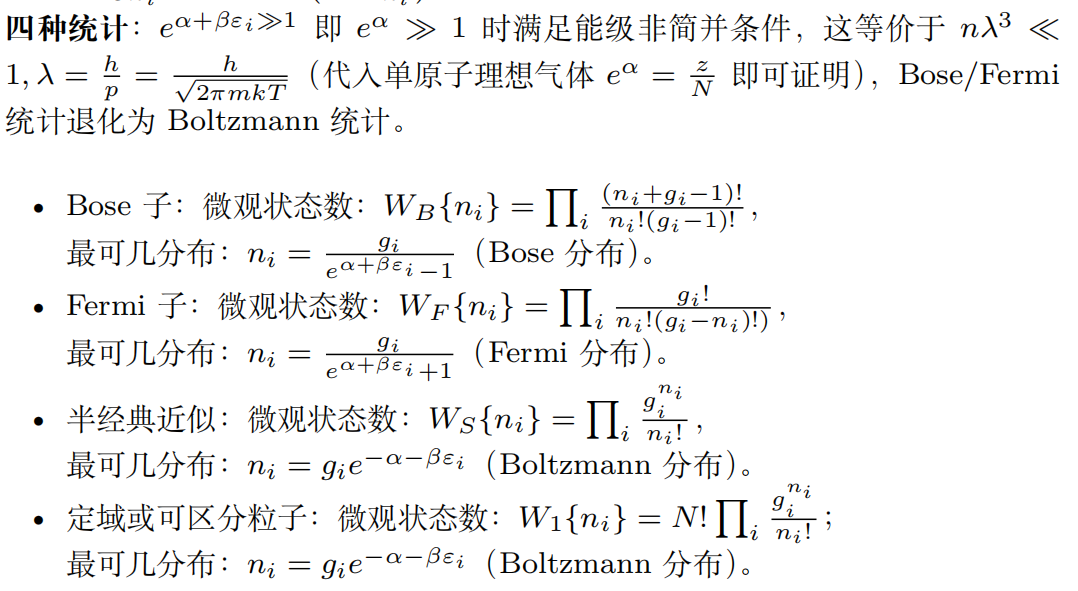
\includegraphics[width=0.33\textwidth]{images/1.png}
    \vspace{-0.6cm}
\end{figure}

\bluetext{配分函数}:定义配分函数$z=\sum_i g_i e^{-\beta\varepsilon_i}$

\begin{figure}[H]
    \vspace{-0.3cm}
    \centering
    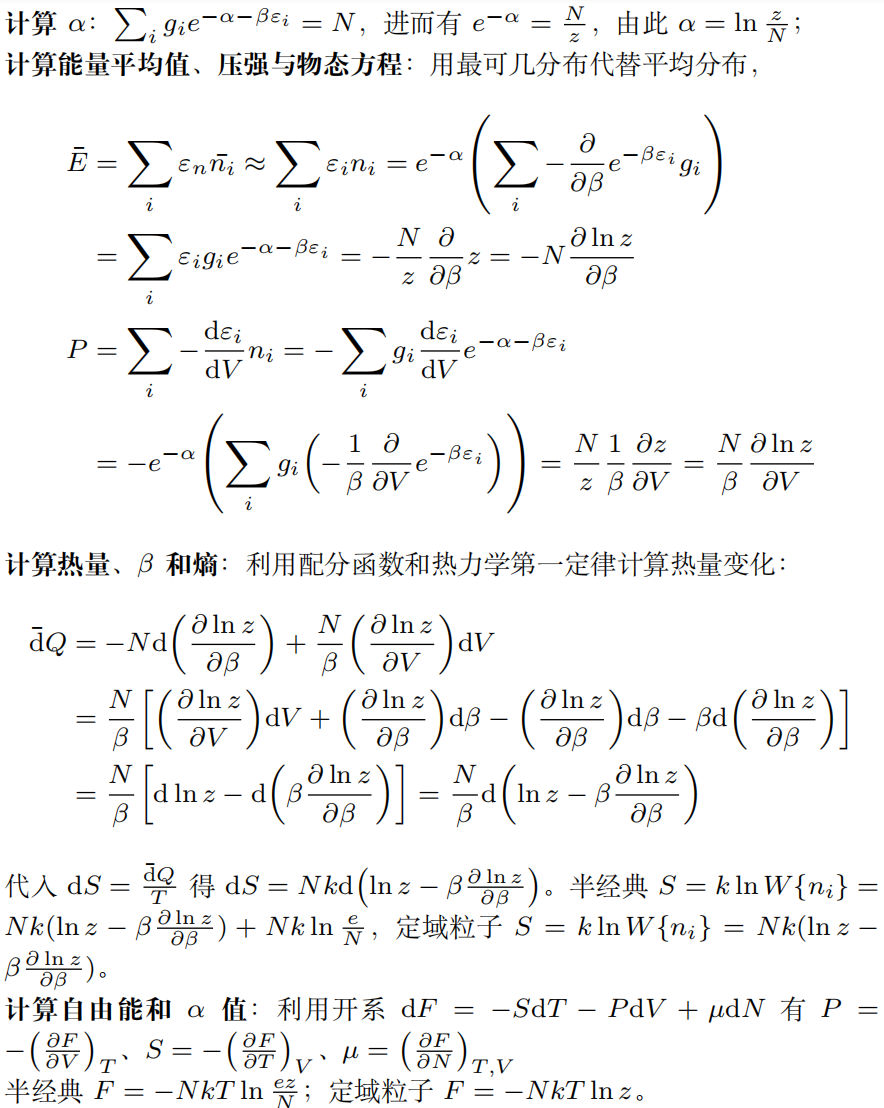
\includegraphics[width=0.33\textwidth]{images/2.png}
    \vspace{-0.6cm}
\end{figure}

\bluetext{熵统计意义}:$\mathrm{d}S = k\mathrm{d}(\ln W_{sm}\{n_i\})$,$S = k\ln W_s\{n_i\}$

推导过程:先有 $\overline{\mathrm{d}Q} = \frac{N}{\beta}\mathrm{d}(\ln z - \beta\frac{\partial\ln z}{\partial\beta})$,再根据 $\ln W_{sm}\{n_i\} = \sum_i (n_i\ln g_i - \ln n_i!)|_{n_i=g_i\exp\{-\alpha-\beta\varepsilon_i\}} \approx \sum_i [n_i\ln g_i - n_i(\ln n_i-1)] \approx \sum_i [n_i\ln \frac{g_i}{n_i} + n_i]|_{\frac{g_i}{n_i}=\exp\{\alpha+\beta\varepsilon_i\}} = \sum_i n_i(\alpha + \beta\varepsilon_i + 1) = N\alpha + \beta E + N = N(\ln z - \beta\frac{\partial\ln z}{\partial\beta}) + N(1-\ln N)$,两边乘 $k$ 对比即得。
\end{multicols}
\end{document}